\chapter{Results}
This chapter will focus on presenting and discussing the results of selected implementations. First part will discuss measured times and its dependency on size and density of the file, number of dimensions and number of pattern matches. For this task, 8 testing files were generated using the Gaussian generating script. Second part will focus on explaining memory usage and also demonstrates the quality of chunking algorithm.

\section{Time complexity}
Time measuring was done with the help of boost library, which belongs in the C++ standard since 2011. In the first graph \ref{fig_compT} there can be seen times of all implemented algorithms achieved for the input file with standard parameters and standard pattern of size $16\times16\times16$. This standard file was compared with all other files and its parameters were:
\begin{itemize}
\item size -- 256 MB
\item density -- 50 \%
\item number of dimensions -- 3
\item presence of pattern -- 0.1 \%
\end{itemize}

Abbreviations on the x axis correspond with these algorithms:
\begin{itemize}
\item BE -- Brute Force for exact pattern matching (EPM)
\item SE -- Baeza-Yates and Navarro algorithm (EPM)
\item BA -- Brute Force for approximate pattern matching (APM)
\item FFS -- Fast Filter Searching (APM)
\item SF -- Stricter Filter (APM)
\item HS -- Hashed Stricter Filter (APM)
\item HS1 -- Hashed Stricter Filter second implementation (APM)
\item HR -- Hashed Stricter Filter third implementation (APM)
\end{itemize}

Yellow color symbolizes the time needed for finishing of preverification and red color means the time of dynamic check.

\begin{figure}
\centering
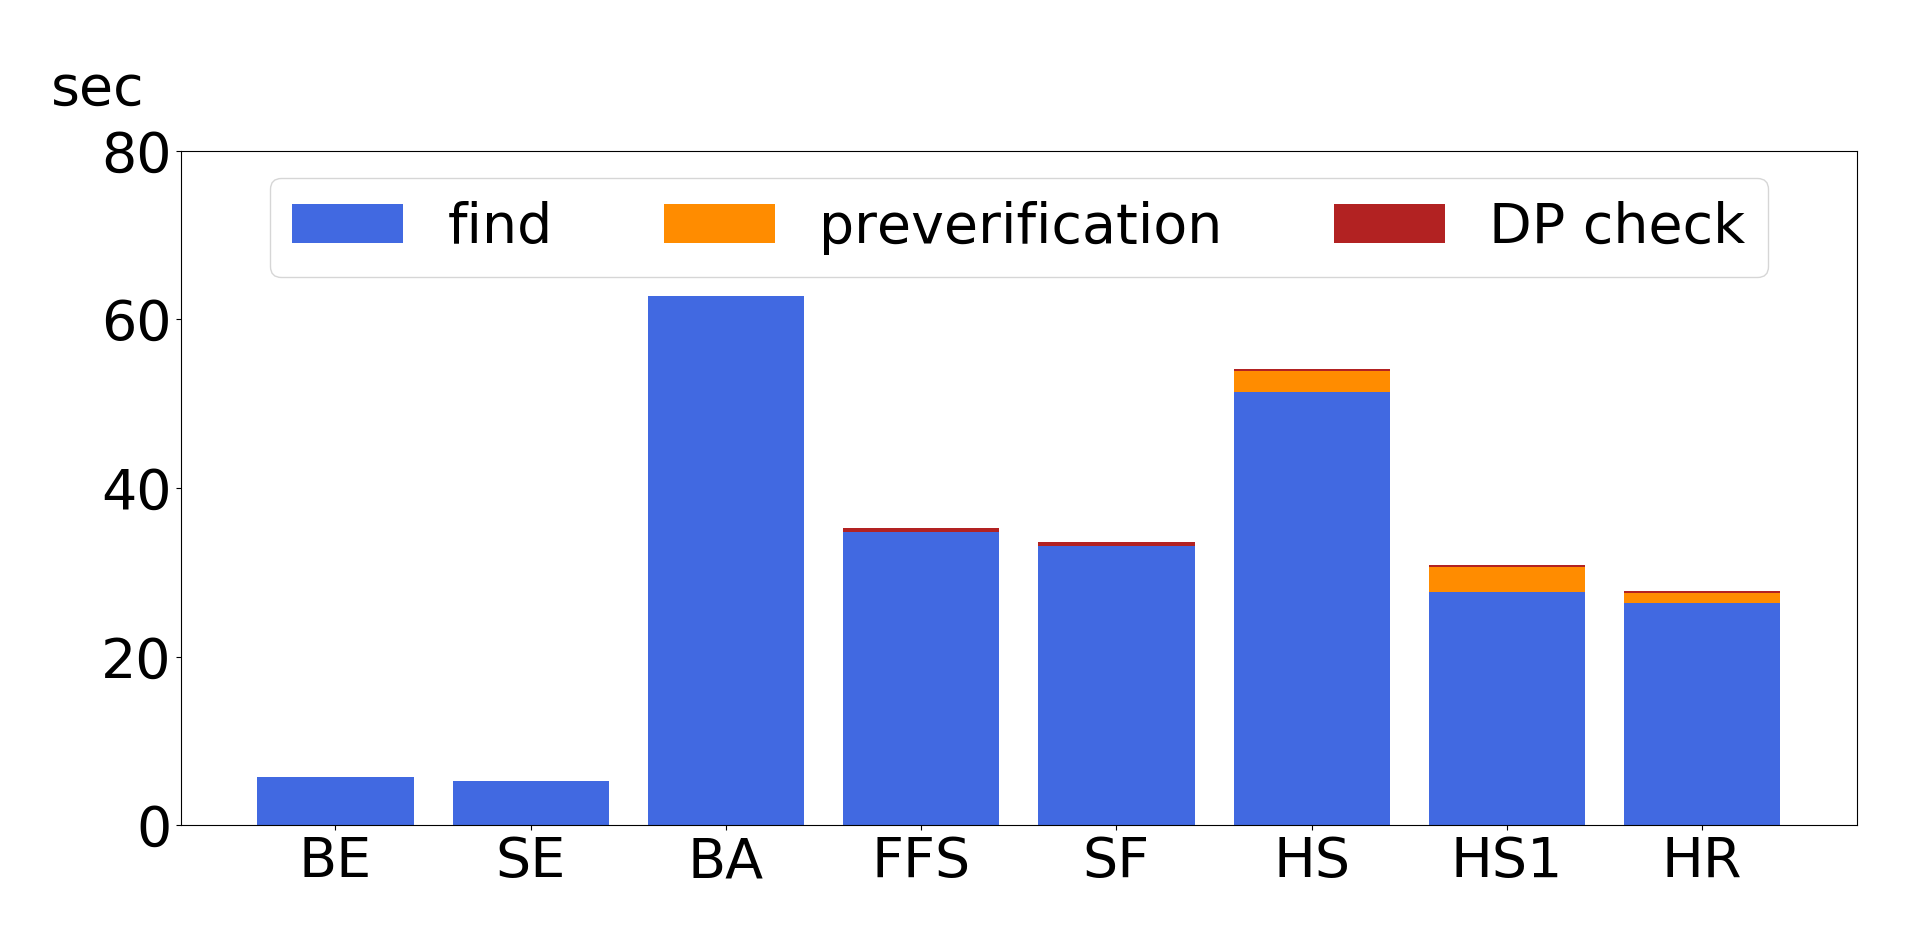
\includegraphics[width=0.8\textwidth]{img/baseAll}
\caption{Computation time for all implemented algorithms.}
\label{fig_compT}
\end{figure}

As can be seen in the graph, solutions of EPM achieve higher performance than APM solutions. This is because whenever exact algorithms encounter a mistake they can dismiss this possible solution while approximate approach has to control until $k$ mistakes are found. Because of this distinct difference exact algorithms are not considered in another graphs.

Another important thing to notice in the graph is that using the preverification before dynamic check visibly speeds up the whole control process, which is a difference between FFS and SF algorithms. 
%to je teda pekna blbost, protoze tam neni zadna preverifikace...zluta je preverifikace..melo by to byt stejny, asi jen chyba mereni

\subsection{Dependency on data density}
Measuring in this section was done using 3 different files. One of them is the standard file specified in the first section, other 2 files were different only in the density of generated data and its values were $100 \%$ and $2 \%$.

In the graph \ref{fig_densRes}, green color represents dense data, orange $50 \%$ density and blue $2 \%$ density. It is clearly visible that lesser the maximum error allowed the higher the dependency on the data density. Times achieved when allowing up to 4 errors is multiple times worse for the least dense data. This happens because when the density is low there is a lot of positions to check even when there are no data in them. 

However there can be seen that solutions using hashes can reach better times than other algorithms especially in the data with low density. Reason for this is that non-hash algorithms can take a while to reach a position with no data, but when using second and third implementation the overall comparison is quicker because the value of the hash is NULL if some of its value is not in the data. Which means that a lot more positions can be skipped directly.

Solution using variant of LSB hash can be very successful for low errors allowed but rapidly worsens with growing error rate. This is why there is such a peak for error 16 and also its time is not used in the last graph for better scaling. In the last graph the brute solution is also omitted.

\begin{figure}
\begin{minipage}{.5\linewidth}
\centering
\subfloat{\label{dens:a}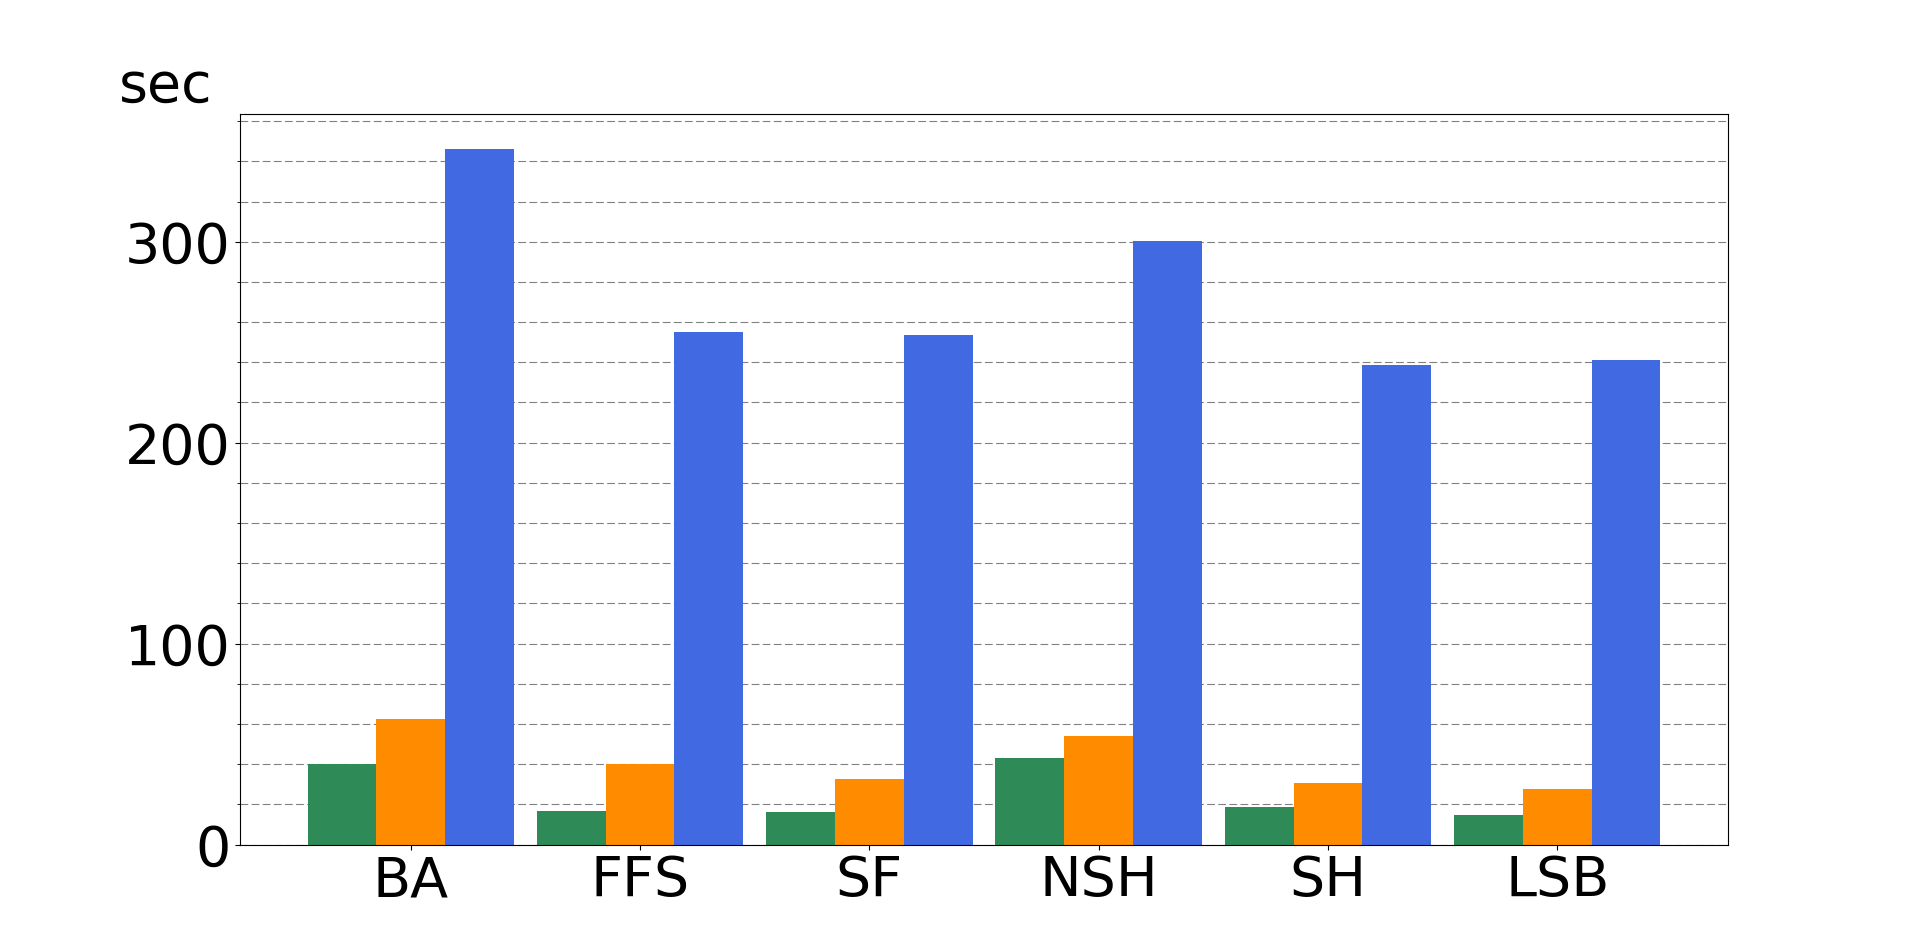
\includegraphics[width=\textwidth]{img/dens0}\caption*{Error = 0}}
\end{minipage}%
\begin{minipage}{.5\linewidth}
\centering
\subfloat{\label{dens:b}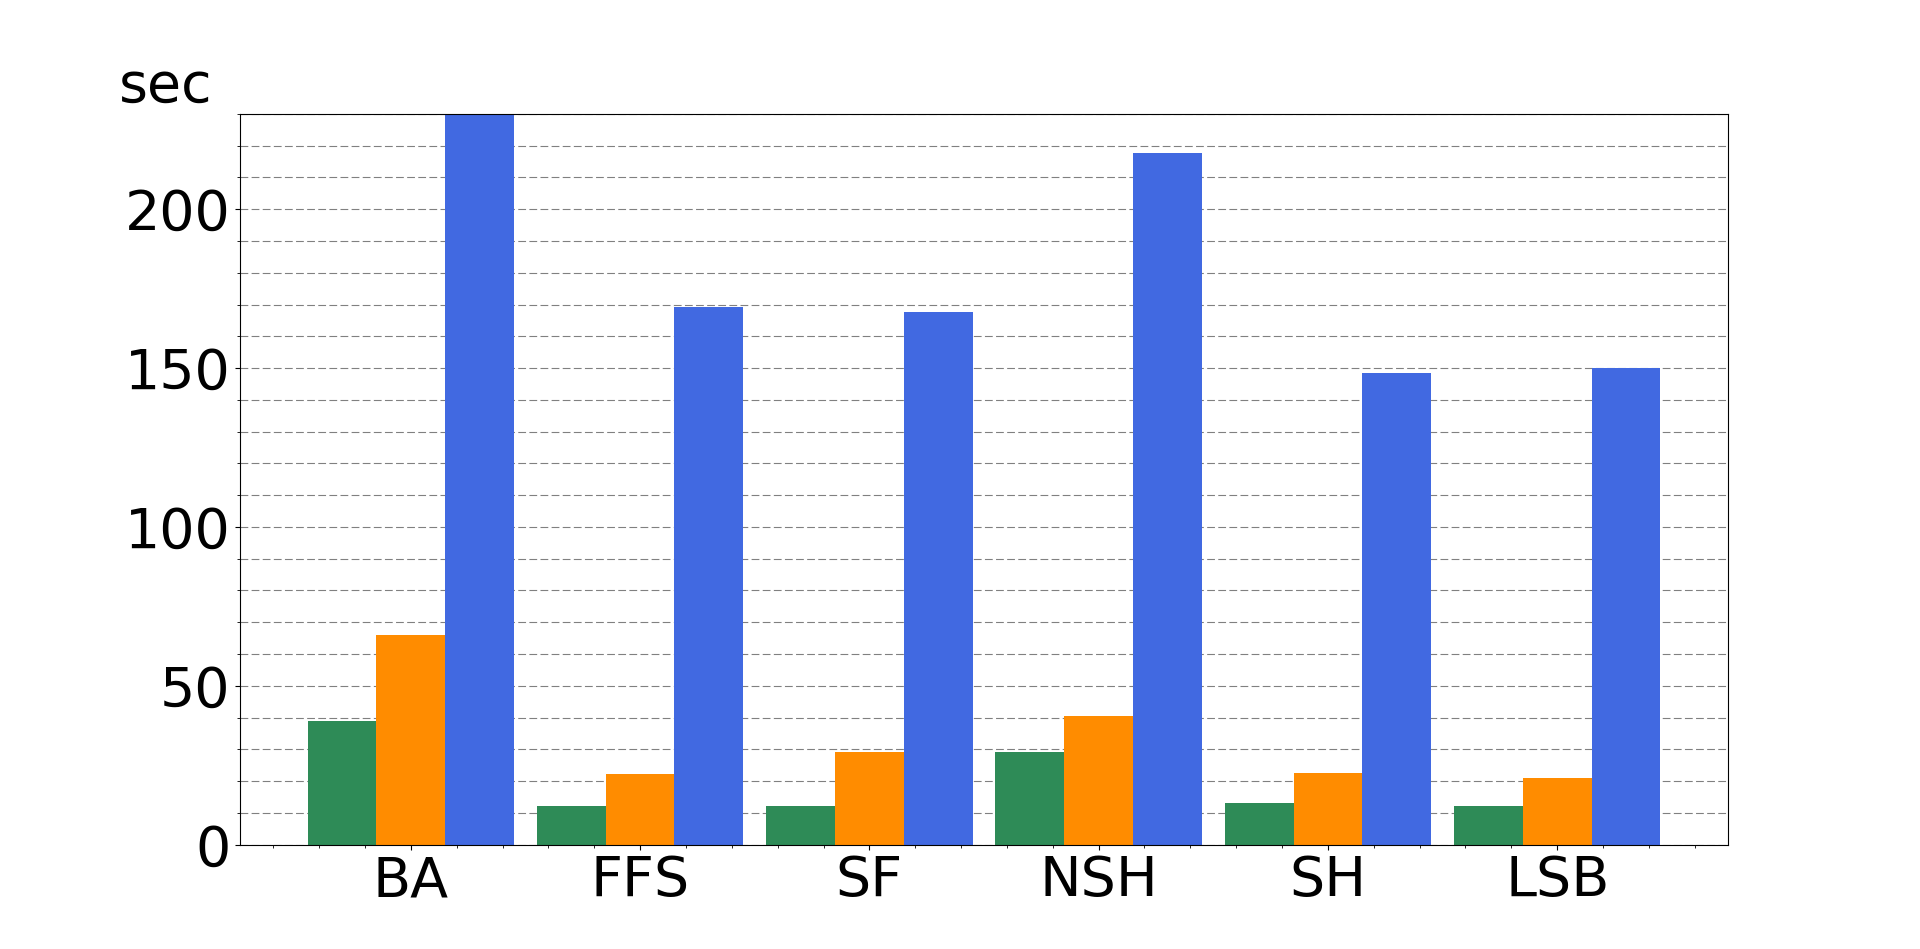
\includegraphics[width=\textwidth]{img/dens4}\caption*{Error = 4}}
\end{minipage}\par\medskip

\begin{minipage}{.5\linewidth}
\centering
\subfloat{\label{dens:c}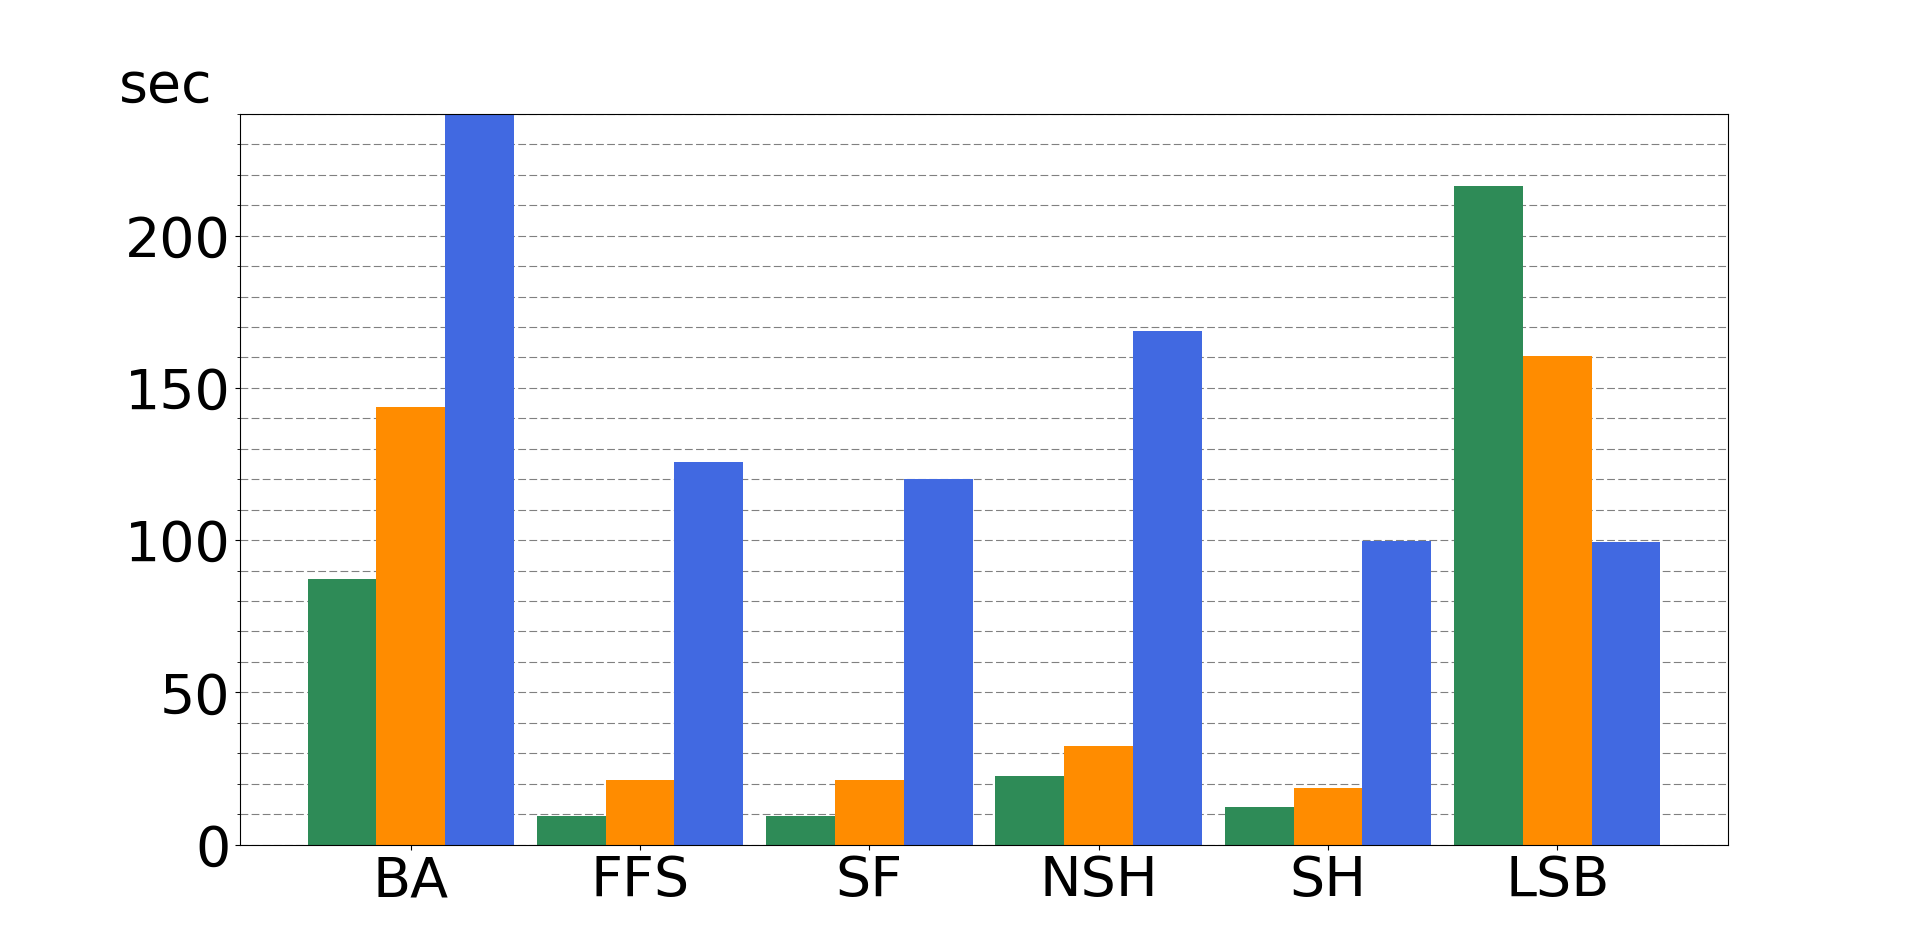
\includegraphics[width=\textwidth]{img/dens16}\caption*{Error = 16}}
\end{minipage}%
\begin{minipage}{.5\linewidth}
\centering
\subfloat{\label{dens:d}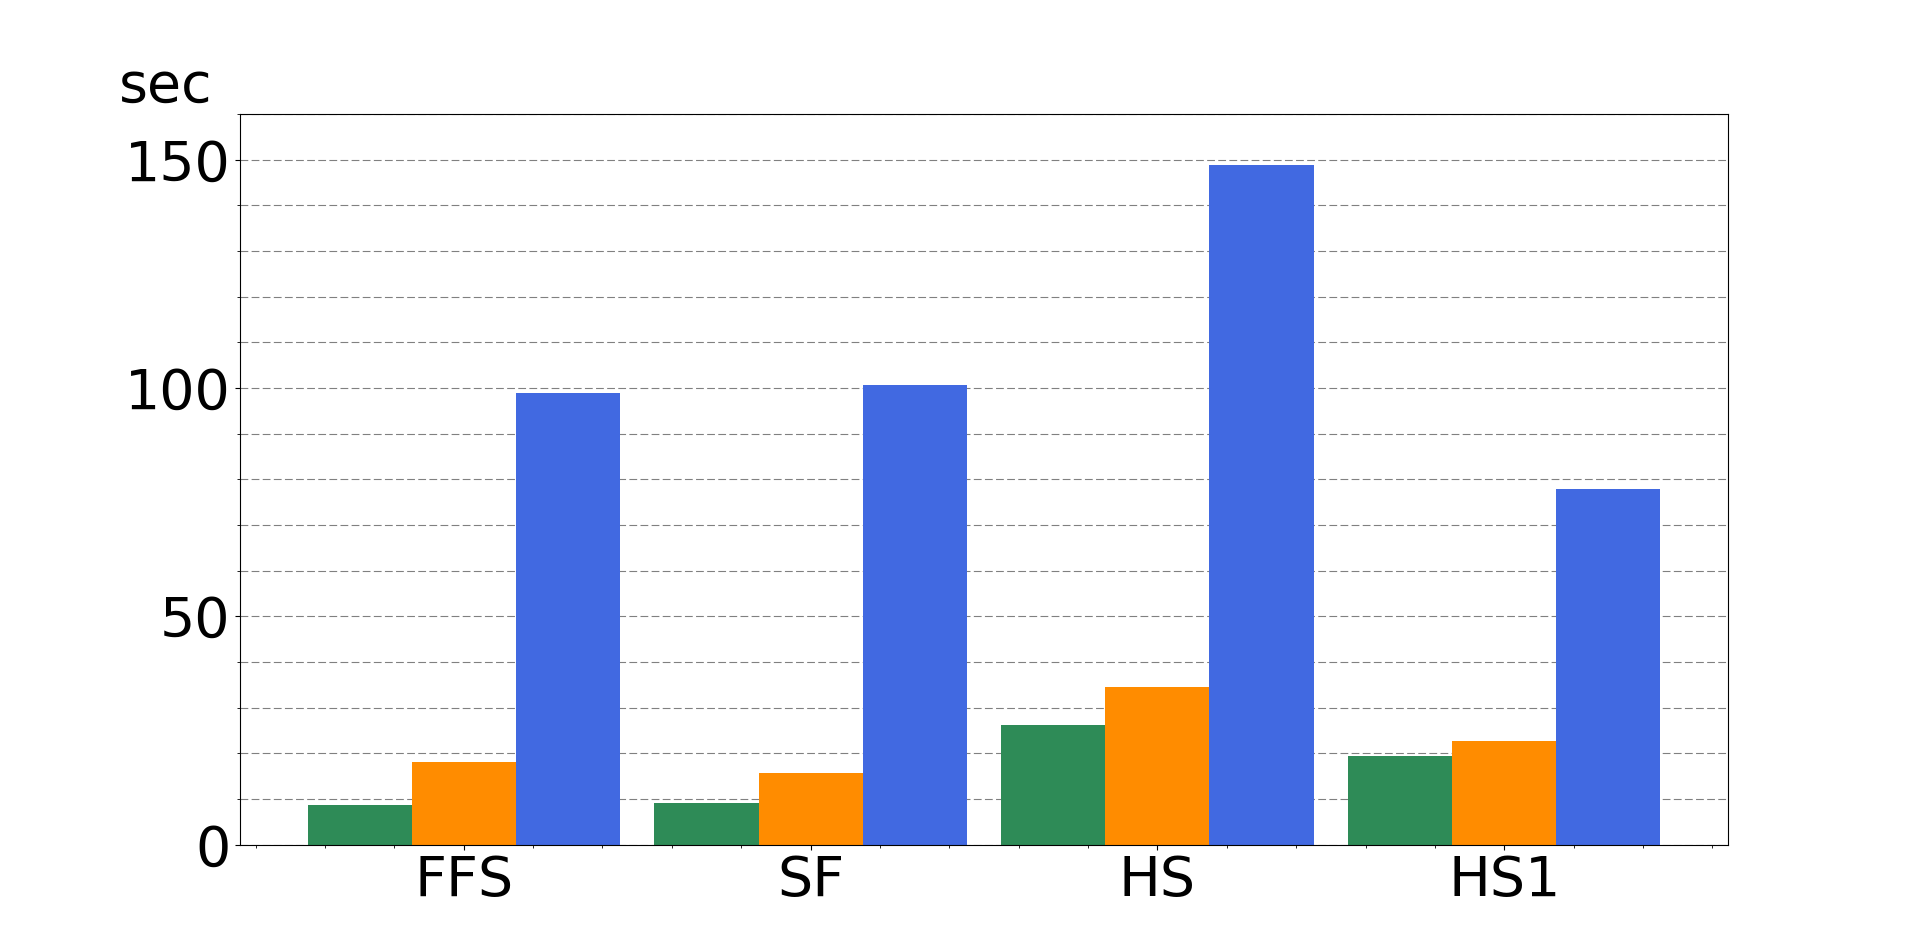
\includegraphics[width=\textwidth]{img/dens64}\caption*{Error = 64}}
\end{minipage}\par\medskip

\caption{Comparison on varying density of data}
\label{fig_densRes}
\end{figure}

\subsection{Dependency on dimensionality}
Three different files were used based on the number of dimensions which were: 2, 3 and 4. In the graph \ref{fig_dimRes} the green color belongs to the 2D file, orange is for the standard 3 dimensional file and blue shows 4 dimensions. It is clear that the bigger the number of dimensions the higher times. This happens because for more dimensions the algorithm gets into higher recursion levels than otherwise.

Second important thing to see in these graphs is that for low error rate and lower dimensionality hash algorithms are way worse than other non-brute solutions. This is caused by a high number of collisions and thus more expensive preverification. Because of the low data dimensionality there is only last dimension of data in the memory that will be hashed which means there is no reusage of already created hashes.

The higher the number of dimensions in chunks the better the reusage rate of hashing algorithms thus better scaling.

\begin{figure}
\begin{minipage}{.5\linewidth}
\centering
\subfloat{\label{dim:a}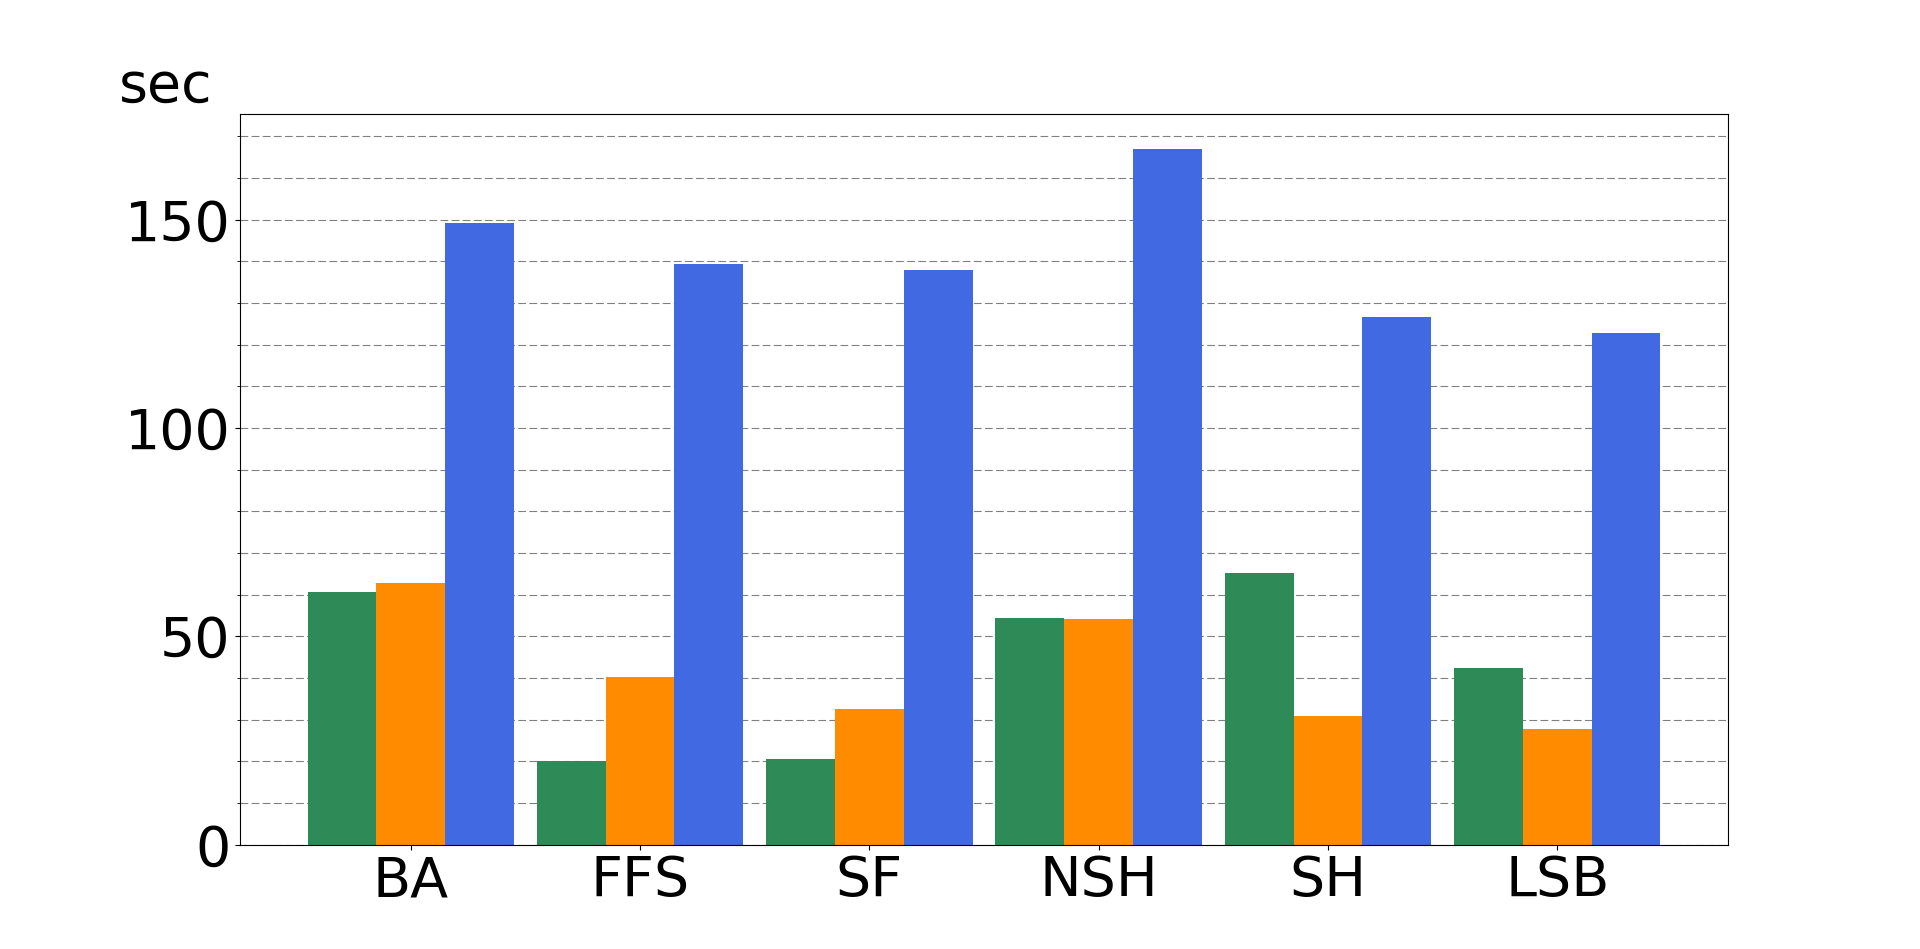
\includegraphics[width=\textwidth]{img/dim0}\caption*{Error = 0}}
\end{minipage}%
\begin{minipage}{.5\linewidth}
\centering
\subfloat{\label{dim:b}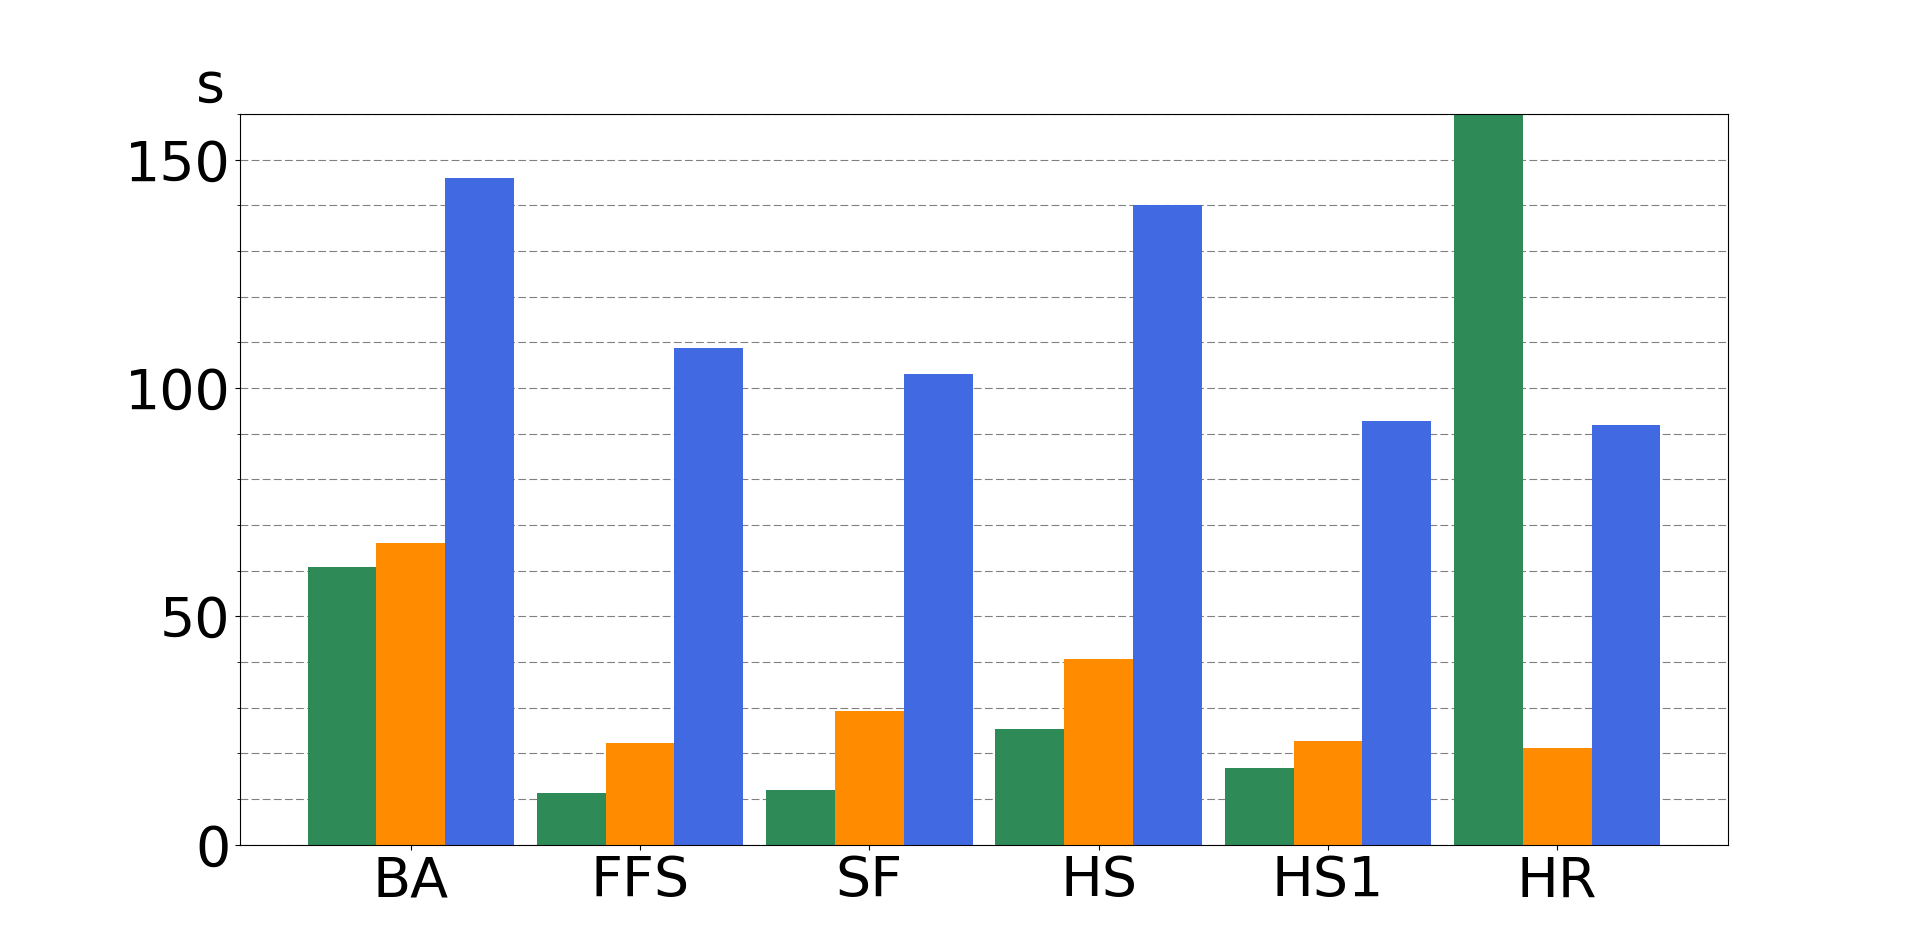
\includegraphics[width=\textwidth]{img/dim4}\caption*{Error = 4}}
\end{minipage}\par\medskip

\begin{minipage}{.5\linewidth}
\centering
\subfloat{\label{dim:c}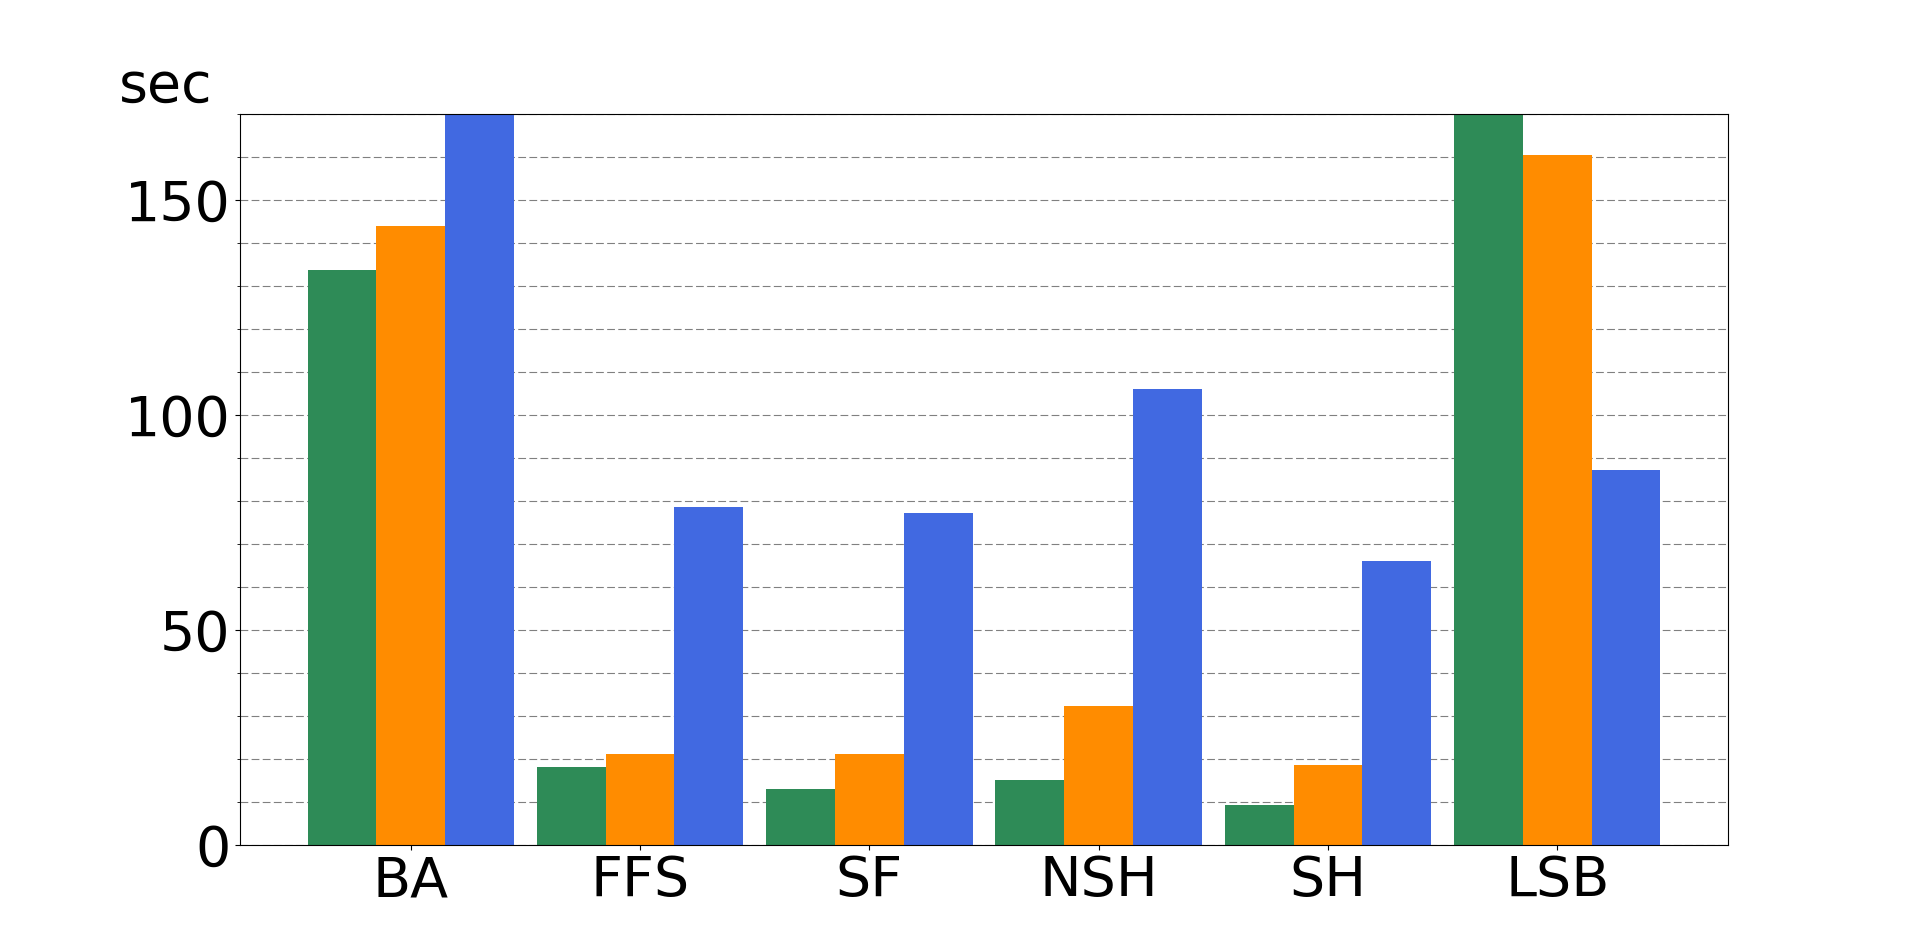
\includegraphics[width=\textwidth]{img/dim16}\caption*{Error = 16}}
\end{minipage}%
\begin{minipage}{.5\linewidth}
\centering
\subfloat{\label{dim:d}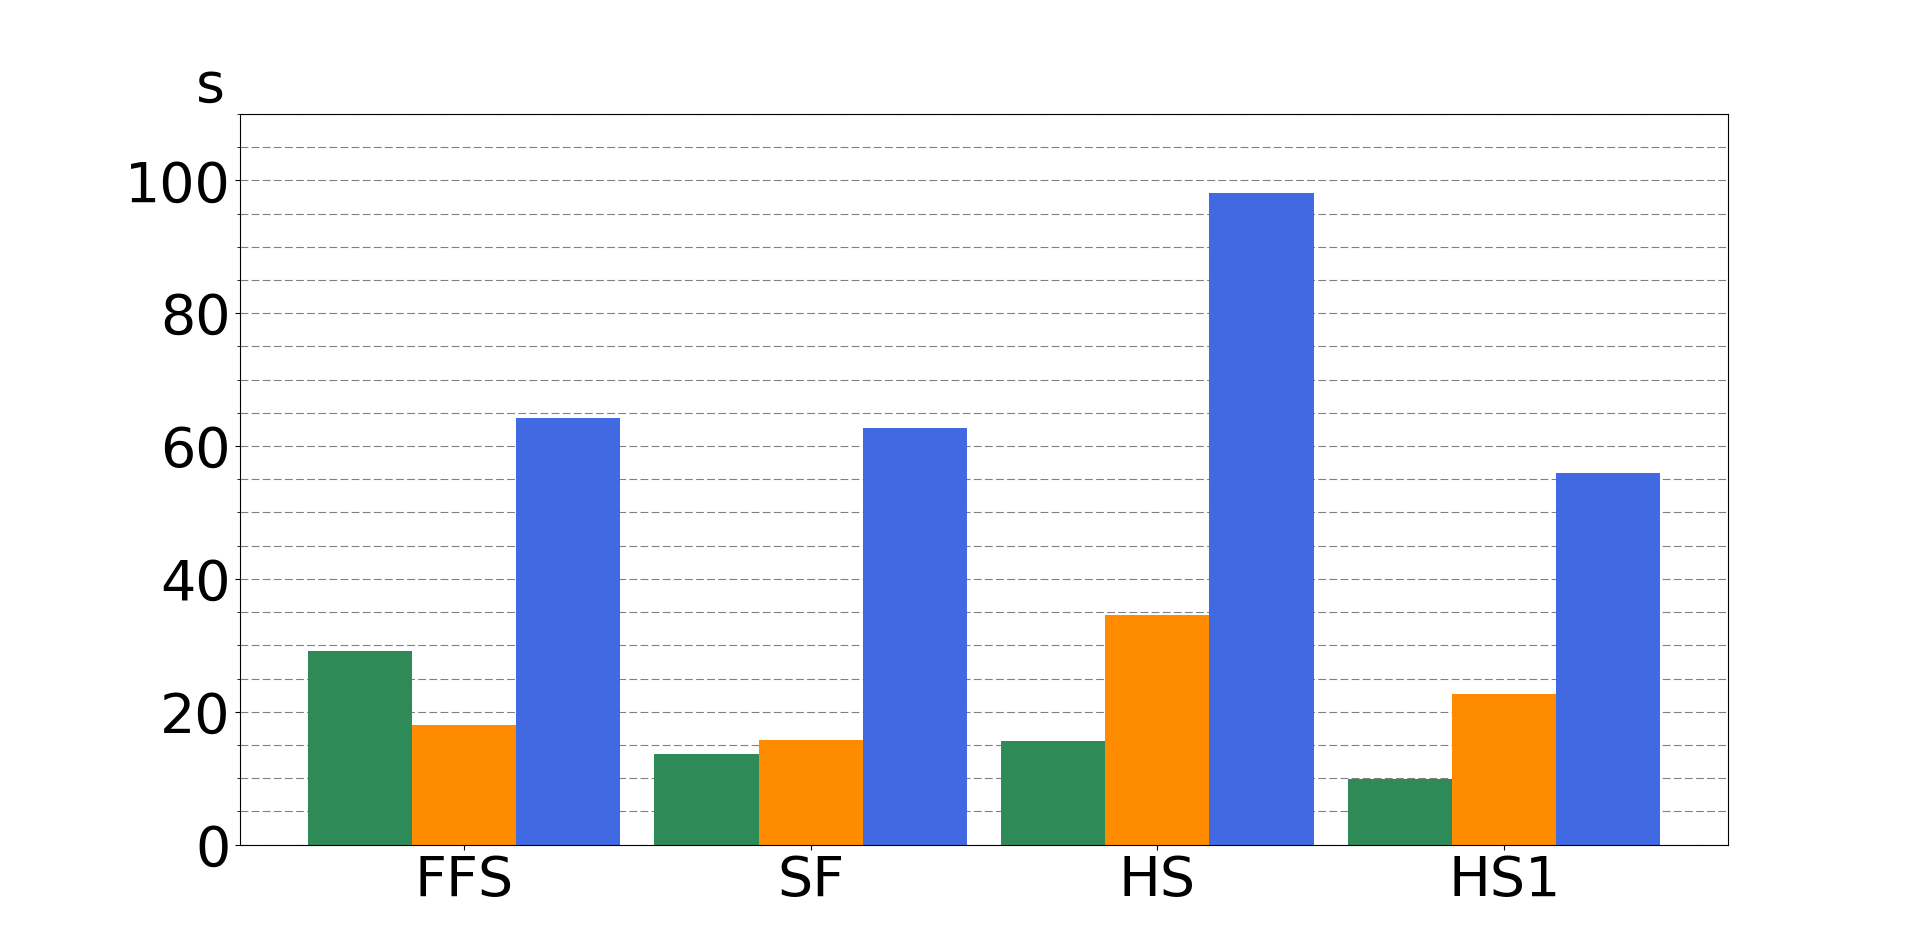
\includegraphics[width=\textwidth]{img/dim64}\caption*{Error = 64}}
\end{minipage}\par\medskip

\caption{Comparison on varying number of dimensions.}
\label{fig_dimRes}
\end{figure}

\subsection{Dependency on frequency of pattern occurrence}
Difference between input files were this time in the number of pattern occurrences. Standard file had the occurrence rate set to $0.1 \%$ while the other two had $1 \%$ and $0.01 \%$. In the figure \ref{fig_patRes} there can be seen only a slight difference in the times of comparing algorithms. This difference is caused only by the preverification step and dynamic checks as they need to control more possible solutions thus lasting longer.

On the other hand, there is nicely illustrated the difference between individual algorithms. 

Stricter Filter algorithm is always slightly better than FFS because preverification step is quicker than dynamic check. Also HS1 is always quicker than HS because there are no repeated hash constructions. Quality of HR is mainly in lower error rates.
%kdyz tam neni zobrazeny nic jinyho muzes se zminit, ze je dobre viditelne porovnani mezi jednolivejma algoritmama - a proc

\begin{figure}
\begin{minipage}{.5\linewidth}
\centering
\subfloat{\label{pat:a}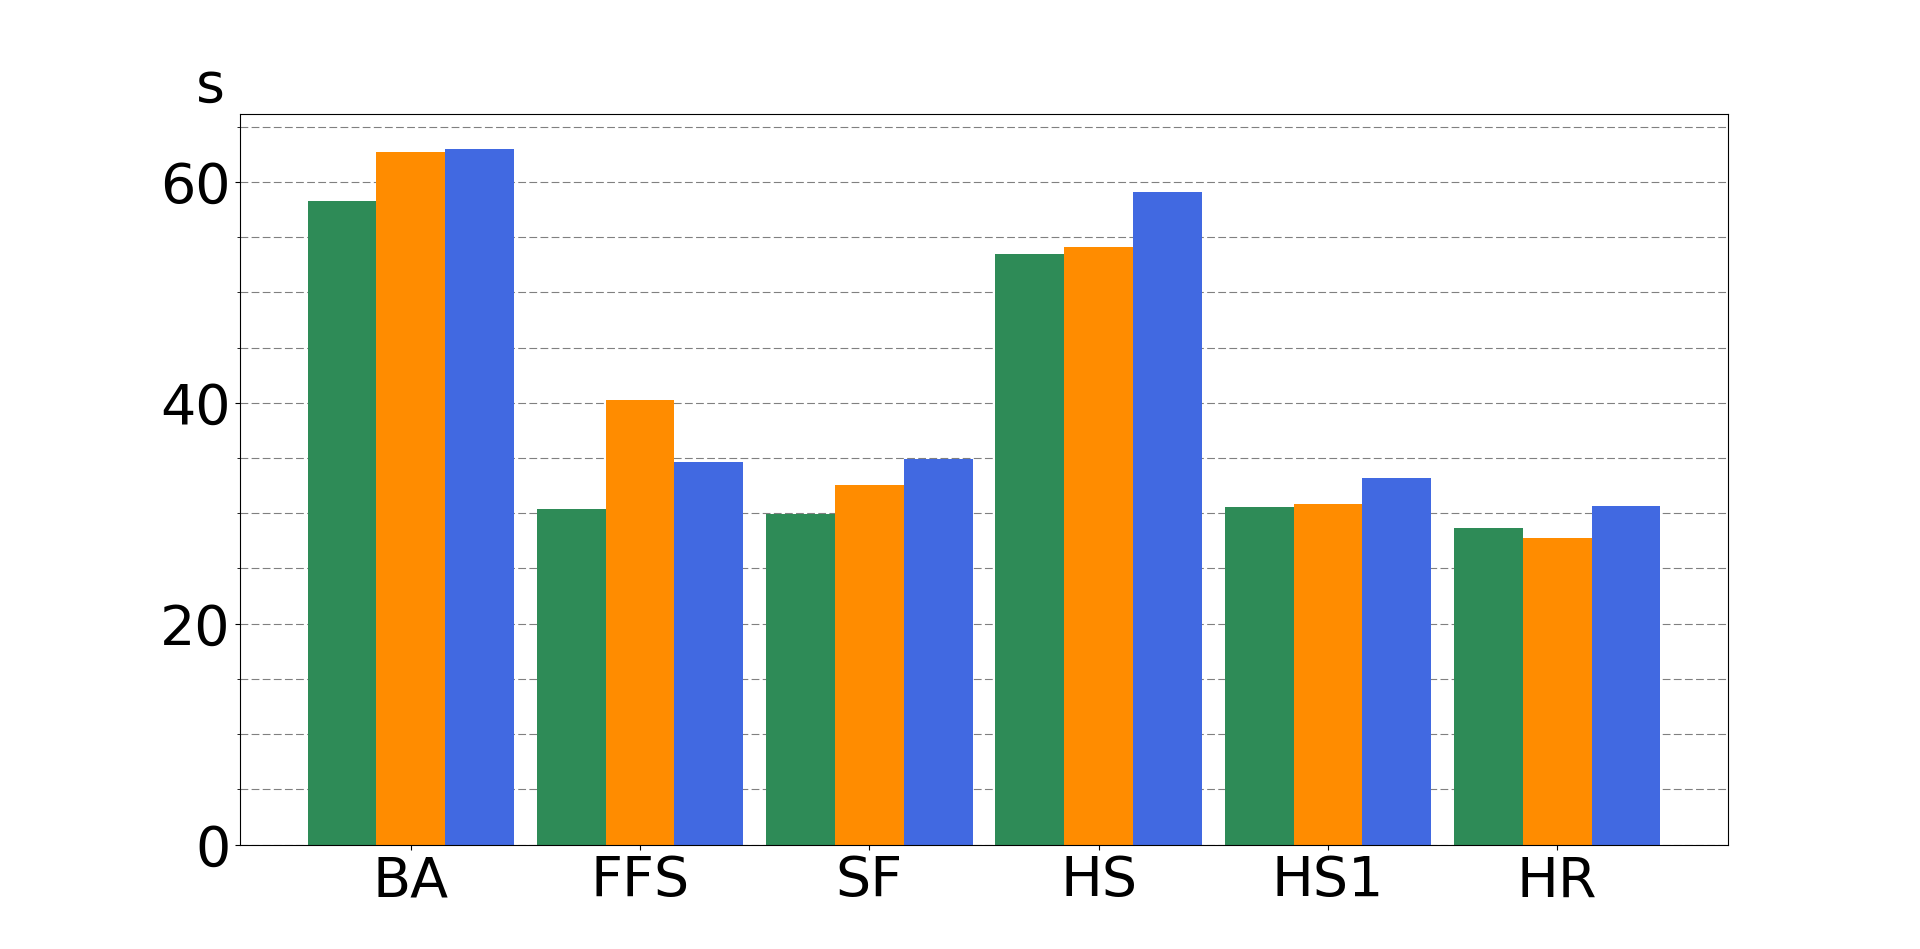
\includegraphics[width=\textwidth]{img/pat0}\caption*{Error = 0}}
\end{minipage}%
\begin{minipage}{.5\linewidth}
\centering
\subfloat{\label{pat:b}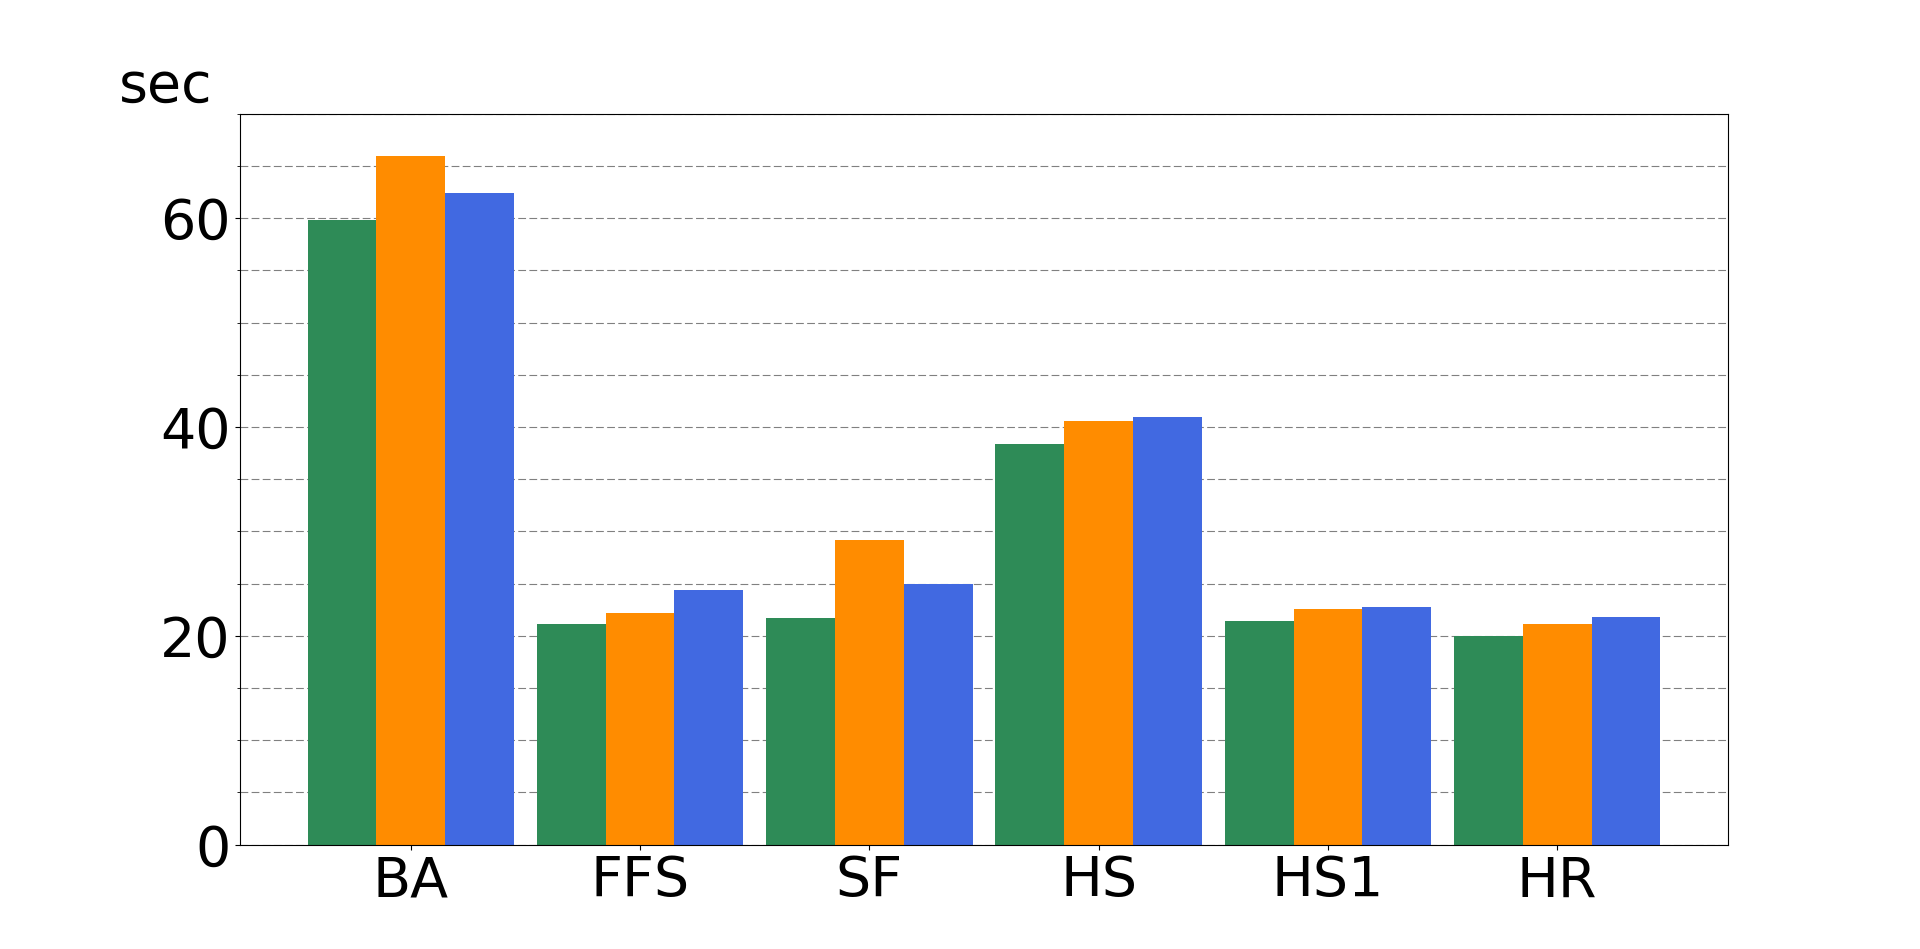
\includegraphics[width=\textwidth]{img/pat4}\caption*{Error = 4}}
\end{minipage}\par\medskip

\begin{minipage}{.5\linewidth}
\centering
\subfloat{\label{pat:c}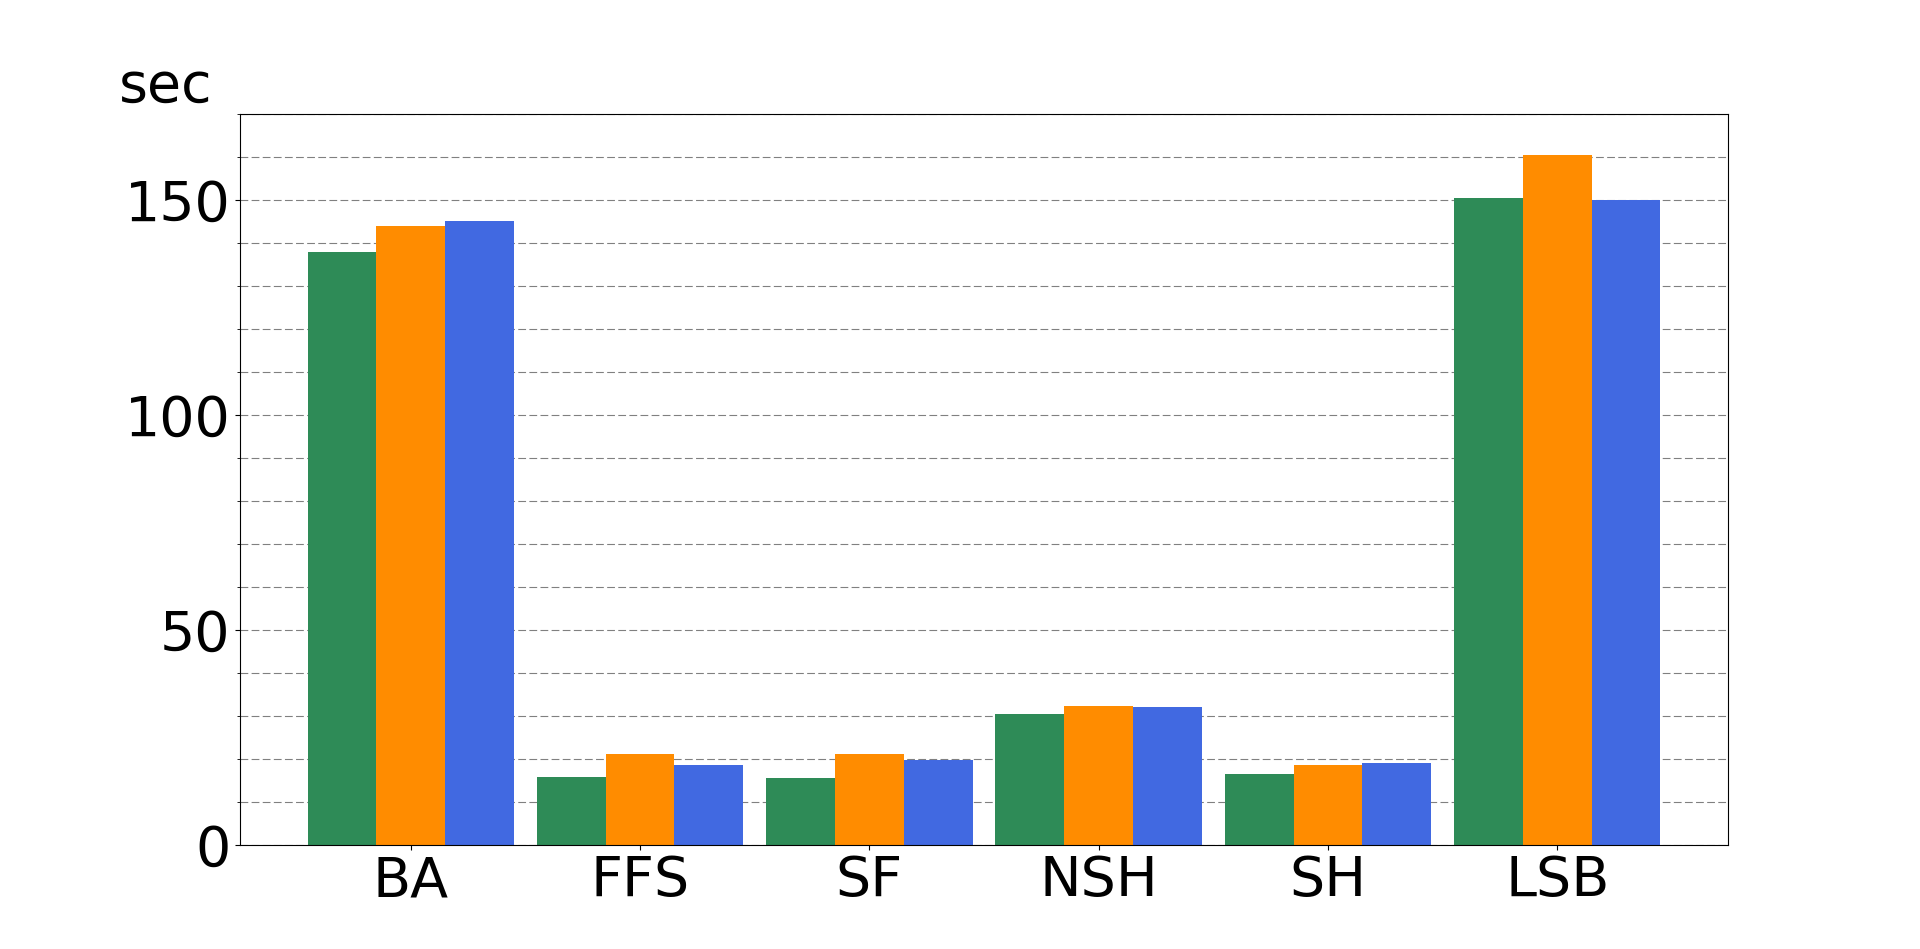
\includegraphics[width=\textwidth]{img/pat16}\caption*{Error = 16}}
\end{minipage}%
\begin{minipage}{.5\linewidth}
\centering
\subfloat{\label{pat:d}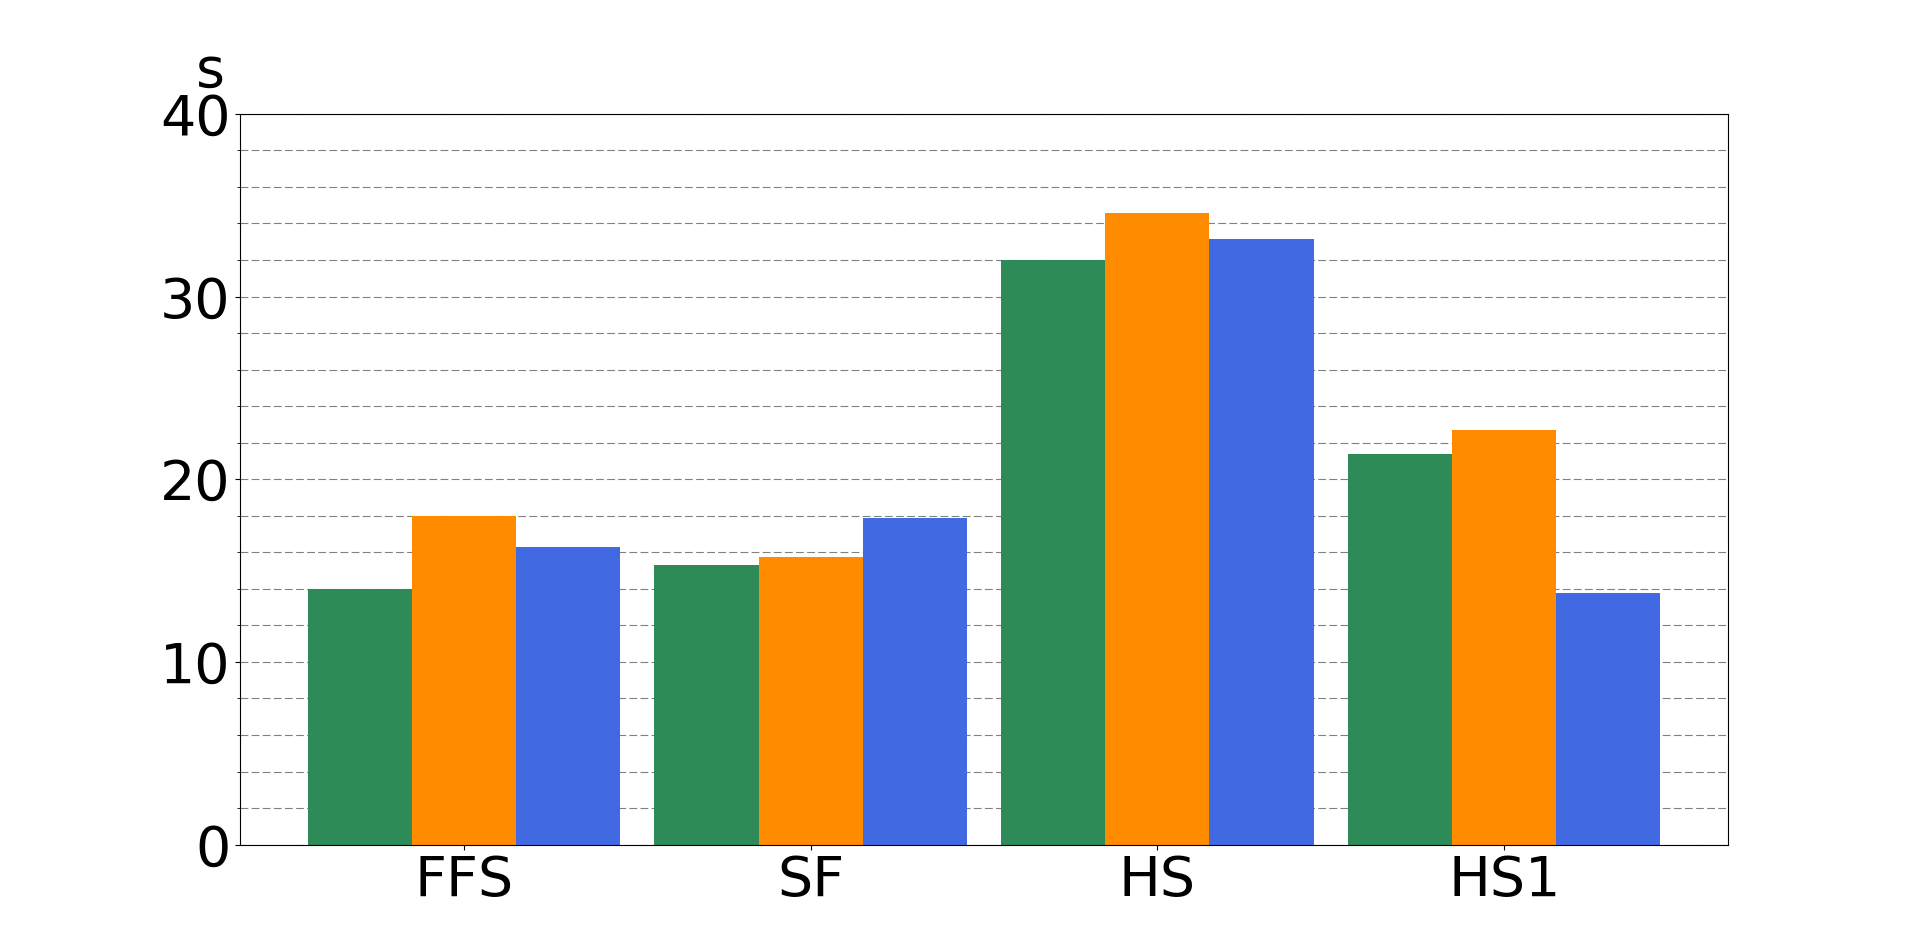
\includegraphics[width=\textwidth]{img/pat64}\caption*{Error = 64}}
\end{minipage}\par\medskip

\caption{Comparison using varying frequency of pattern occurrence.}
\label{fig_patRes}
\end{figure}

\subsection{Dependency on input file size}
In the last graph figure \ref{fig_sizeRes} there can be seen comparison of standard (orange) file and file of the size 4 GB but measured twice, first with the pattern of size $64\times64\times64$ and second with the standard pattern (size $16\times16\times16$).
% a proc patern 64 a 16? - 16 protoze standard a 64 aby to bylo podobnejsi pomerem
% taky ze tam je logaritmicky meritko, aby to bylo lip videt

The difference in the pattern size proved to have only a slight effect on the final reached times. It is no surprise that the times are different. %co to je za zblept? to je snad jasny ze to bude vetsi, ale jestli to je spravne vetsi


\begin{figure}
\begin{minipage}{.5\linewidth}
\centering
\subfloat{\label{size:a}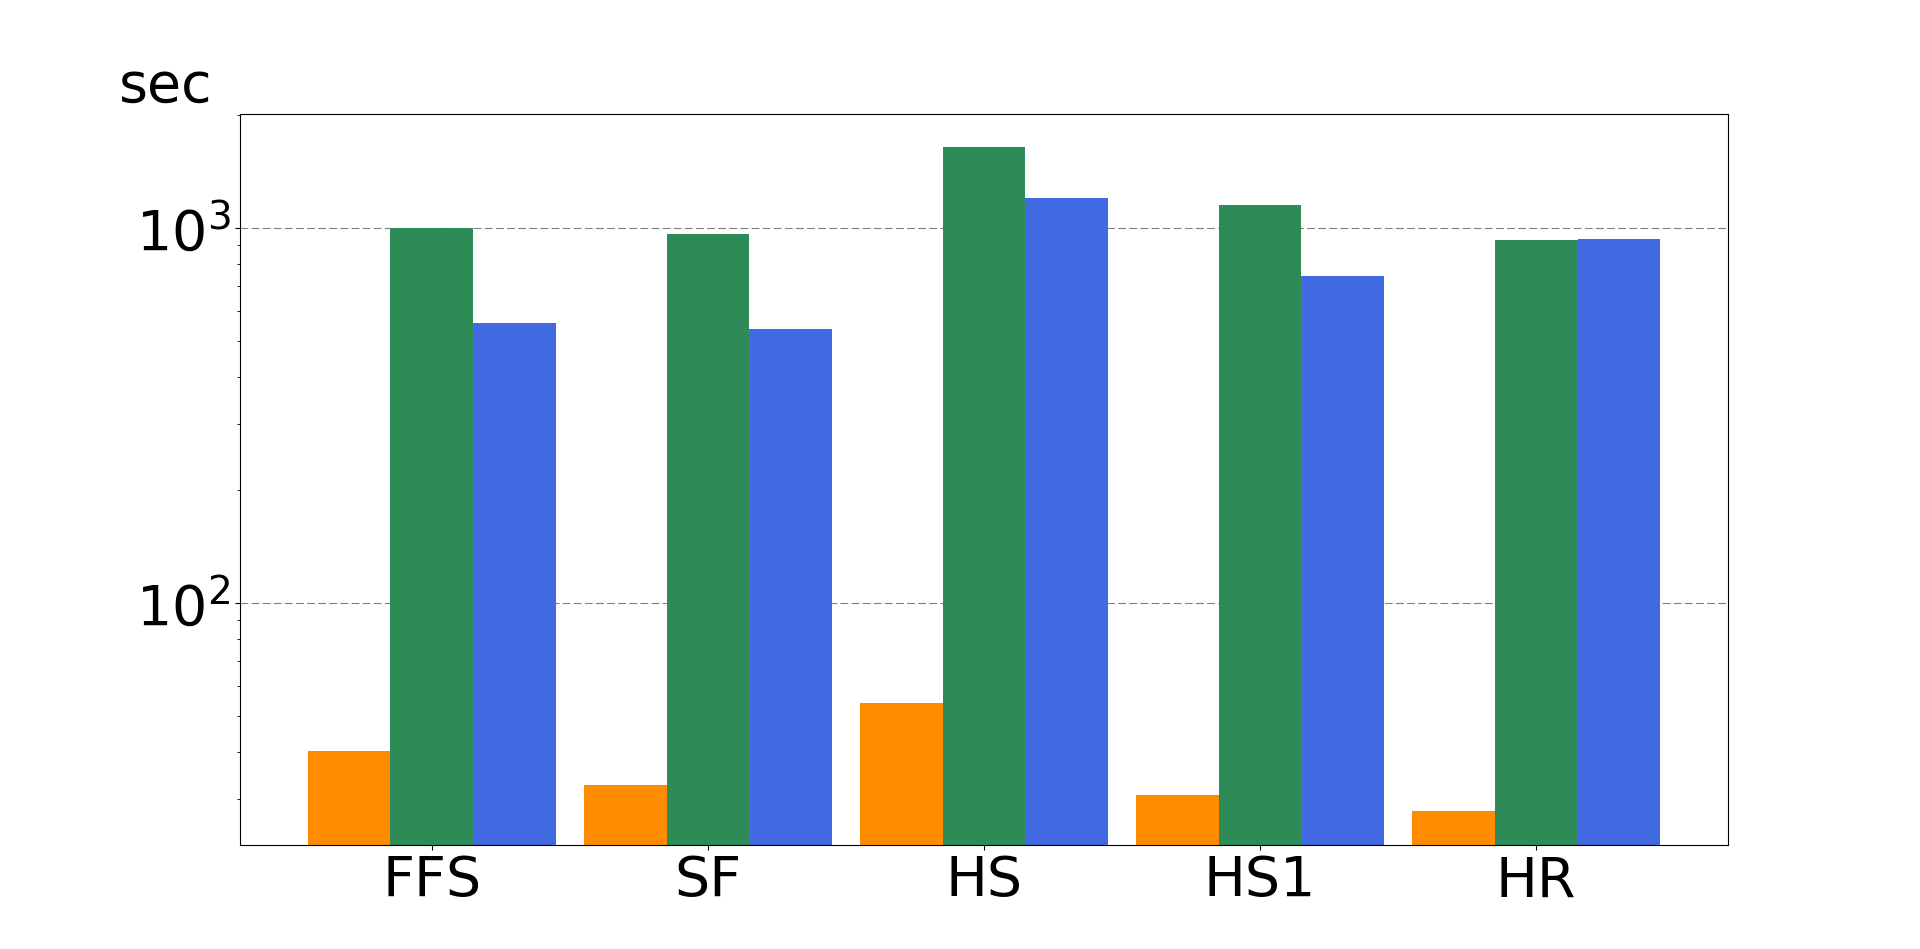
\includegraphics[width=\textwidth]{img/size0}\caption*{Error = 0}}
\end{minipage}%
\begin{minipage}{.5\linewidth}
\centering
\subfloat{\label{size:b}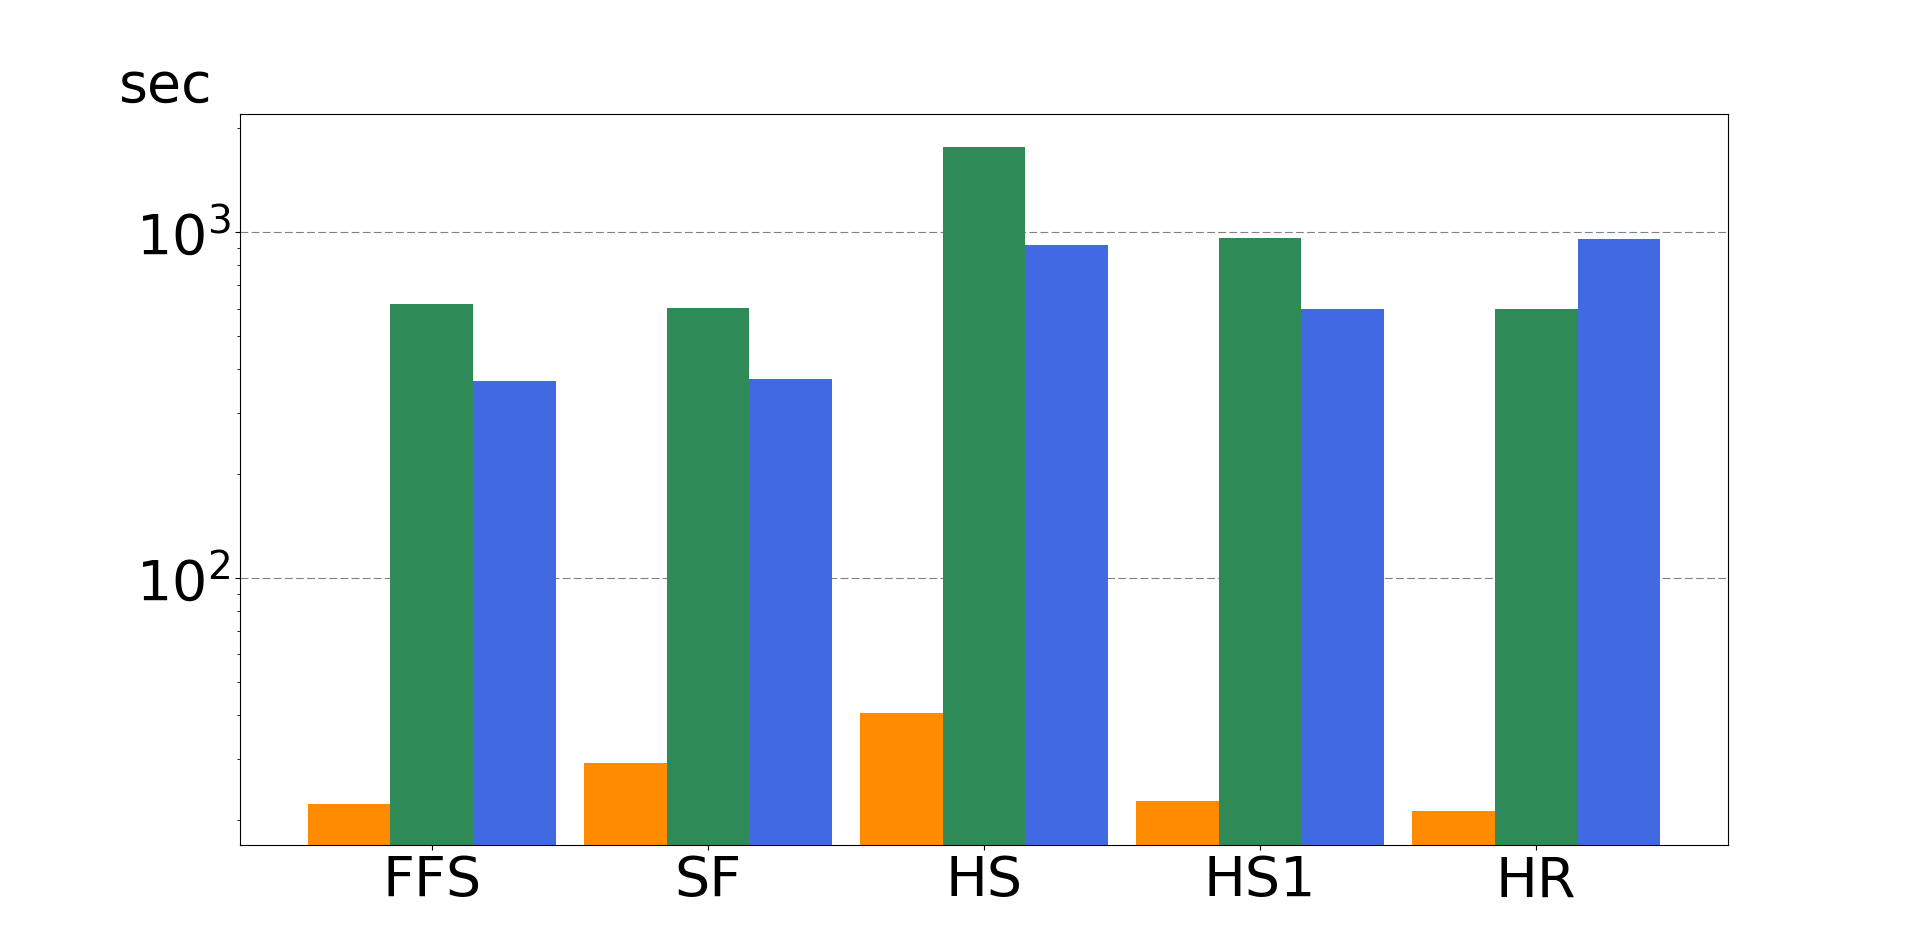
\includegraphics[width=\textwidth]{img/size4}\caption*{Error = 4}}
\end{minipage}\par\medskip

\begin{minipage}{.5\linewidth}
\centering
\subfloat{\label{size:c}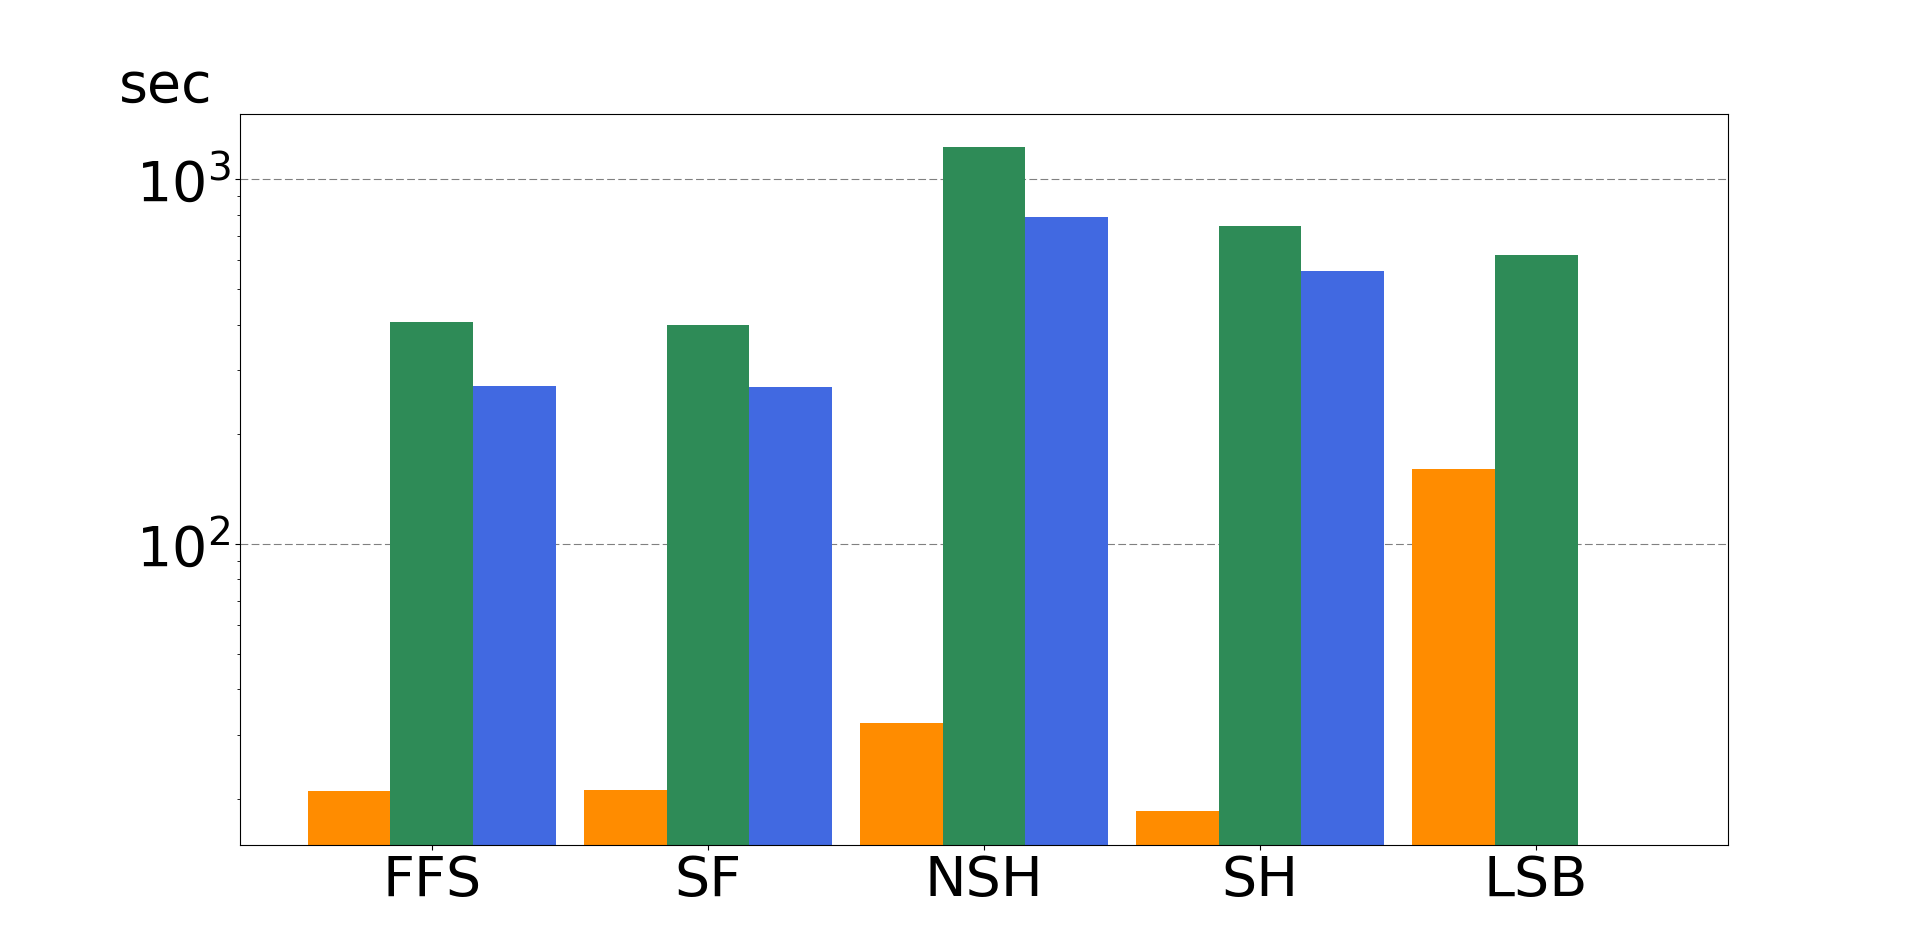
\includegraphics[width=\textwidth]{img/size16}\caption*{Error = 16}}
\end{minipage}%
\begin{minipage}{.5\linewidth}
\centering
\subfloat{\label{size:d}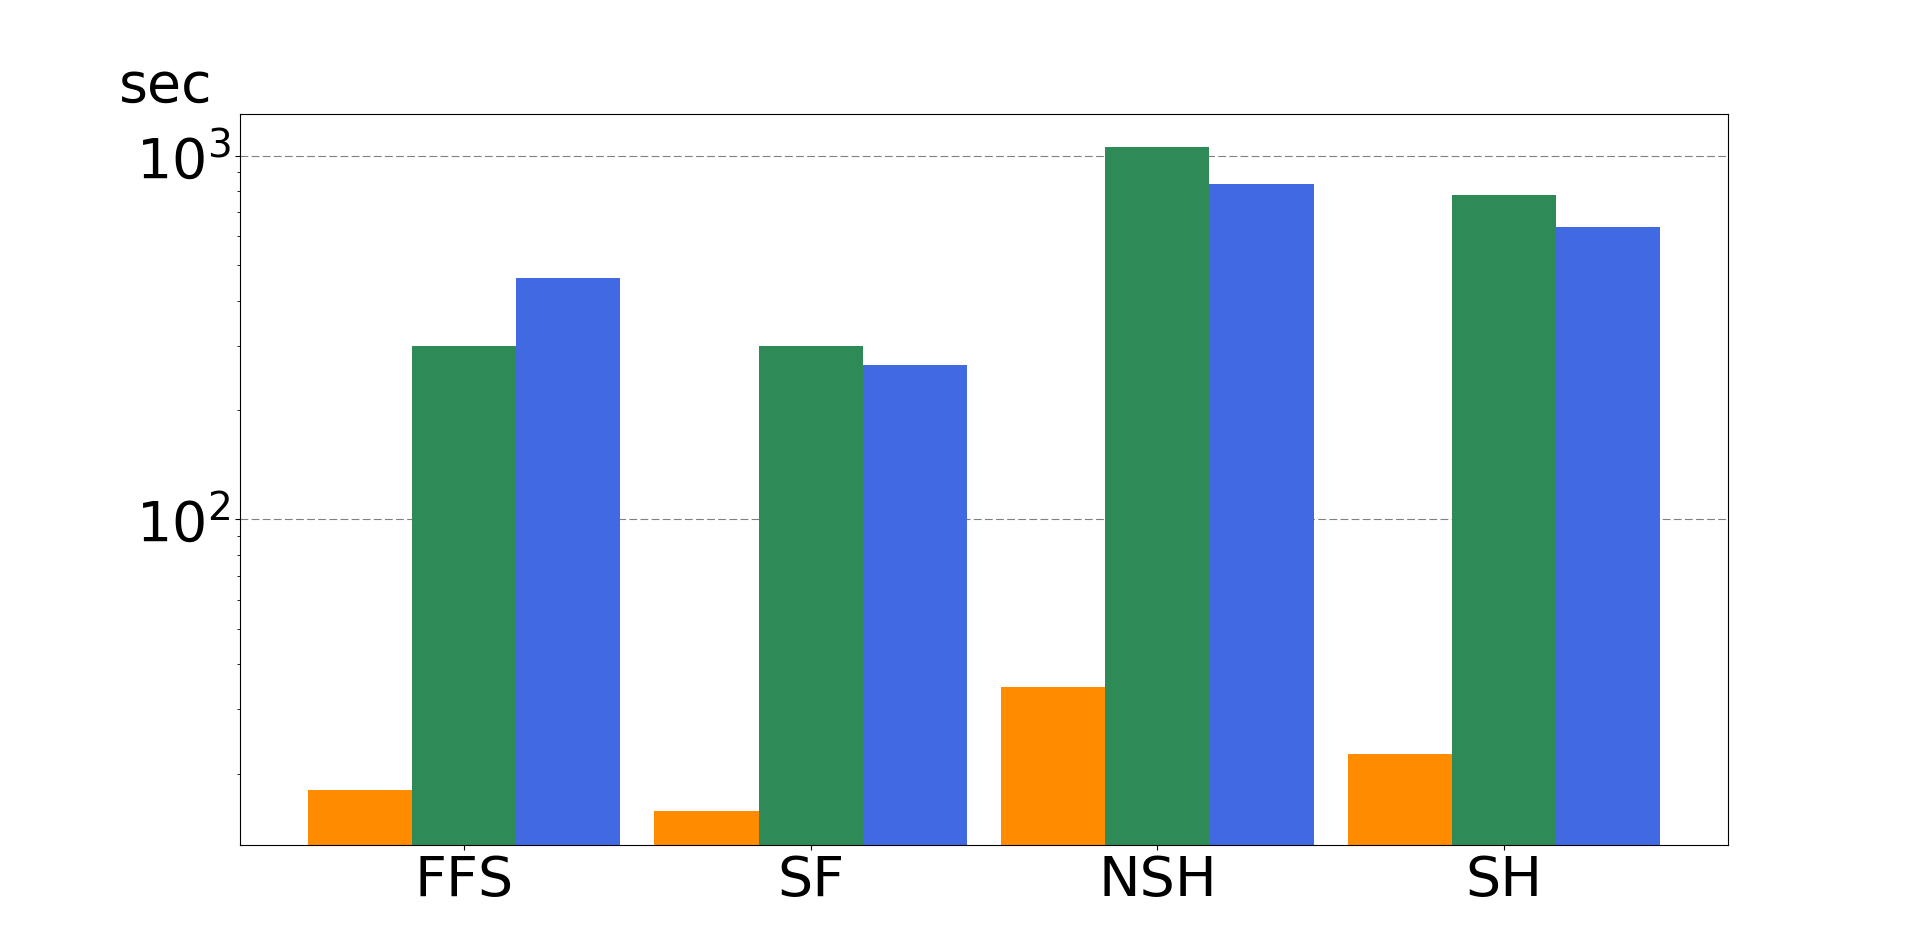
\includegraphics[width=\textwidth]{img/size64}\caption*{Error = 64}}
\end{minipage}\par\medskip

\caption{Test on 4GB data file.}
\label{fig_sizeRes}
\end{figure}


\subsection{Dependency on error rate}
In all the figures mentioned in previous sections, there can be seen that the higher the error rate the higher the times. This is caused by the course of action of all algorithms used, i.e. they all need to control more data before the maximum number of errors is found. % to plati jen u app brutu...ostatni hledaji identitu a pak se to jen preverifikuje...spis napis treba pocty tech prednalezenejch reseni...ze hash tim trpi ale co to ma zas za vyhody

This is much more obvious when looking only at the hash algorithms, which with the increasing error rate have multiple times higher collision rate and that makes them much worse than Stricter Filter and Fast Filter for high number of errors. However, when approached with low error rate and low density of data they prove to be better solution than Navaro and Baeza-Yates algorithms.
%z jakyho duvodu? (part size - hlavne u rolling hashe) - moznost zmenit pocitani j aby to bralo v uvahu hashovani a nepouzivalo moc maly part sizy

\section{Memory usage}
Implemented solutions uses a cache like memory system with the size of $max(64, m)$ where $m$ is the size of the pattern. This means that when the requested file is not in the memory it will be loaded into cache and if the cache is full the oldest data are discarded. 

When taking brute solution as a base line that uses only cache and pattern memory, FFS and SF algorithms do not use any added memory except for dynamic check that needs only extra space for creating of matrix of size $m\times m$ for the alignment purposes. Algorithms using hashes need extra space for the hashed pattern but the rest of its memory usage is the same as in the SF algorithm because the memory needed in each dimension is $\lceil 2\times n\rceil$ and thus the memory usage is very similar. % tohle nedava moc smysl...proste tam napis ze to zabere radove stejne, a jen ani ne 2krat tolik, protoze se ty hashe ulozi do podobny struktury jako normalni data, jen diky tomu ze to jsou hashe tak je to mensi
%navic vlastne ten prvni hash alg pouziva extra pamet jen na pattern, to tam taky napis

\subsection{Binary chunking}
In the table \ref{tab_chunk} there can be seen how using the binary format affects the size of the used data files. There can be seen that usage of the chunking lowers the size of the file about at least $60 \%$. This is because all the data values fits into 2 bytes and there is no need to store information about the dimensions as it is in the name of the file. 
%there can be seen zni divne a obzvlast 2krat za sebou
%60% je nesmysl..to ze mas zrovna cisla na 60% neznamena ze je to 60% --proste to snizuje o hodne, ale ze to dosta zavisi na densite...kdybys mela dostatecne malou density (promile treba) tak to bude i horsi

Low density data files can not be chunked as effectively because each dimensions contains more values thus the created mask file needs to be much longer.

\begin{table}
\centering
\begin{tabular} {| c | c | c | c |}

\hline
Density (\%) & 100 & 50 & 2 \\
\hline
Size Before (MB) & 239.6 & 235.7 & 284.3 \\
\hline
Size After (MB) & 39.8 & 42.2 & 109.8 \\
\hline
\hline
New Size (\%) & 16.61 & 17.9 & 38.62  \\
\hline
\end{tabular}
\caption{Size of input files before and after chunking.}
\label{tab_chunk}
\end{table}

\section{Real datasets}
Every algorithm was successfully tested on datasets provided on \url{archive.ics.uci.edu/ml/datasets} but the times are not given as the size of the chosen datasets did not allow proper measuring due to its small size. % delsi, vic okecat...proc to neslo zmerit? nepsal bych tam uplne doslova every algorithm ale neco jako, Solutions were tested using some datasets ..... . Most of those are relatively small compared to the testing data, so the measuring bla bla...

\section{Discussion}

